\documentclass{standalone}
\usepackage{tikz}
\usetikzlibrary{patterns, positioning}
\usepackage[sfdefault]{ClearSans} %% option 'sfdefault' activates Clear Sans as the default text font
\usepackage[T1]{fontenc}

\begin{document}
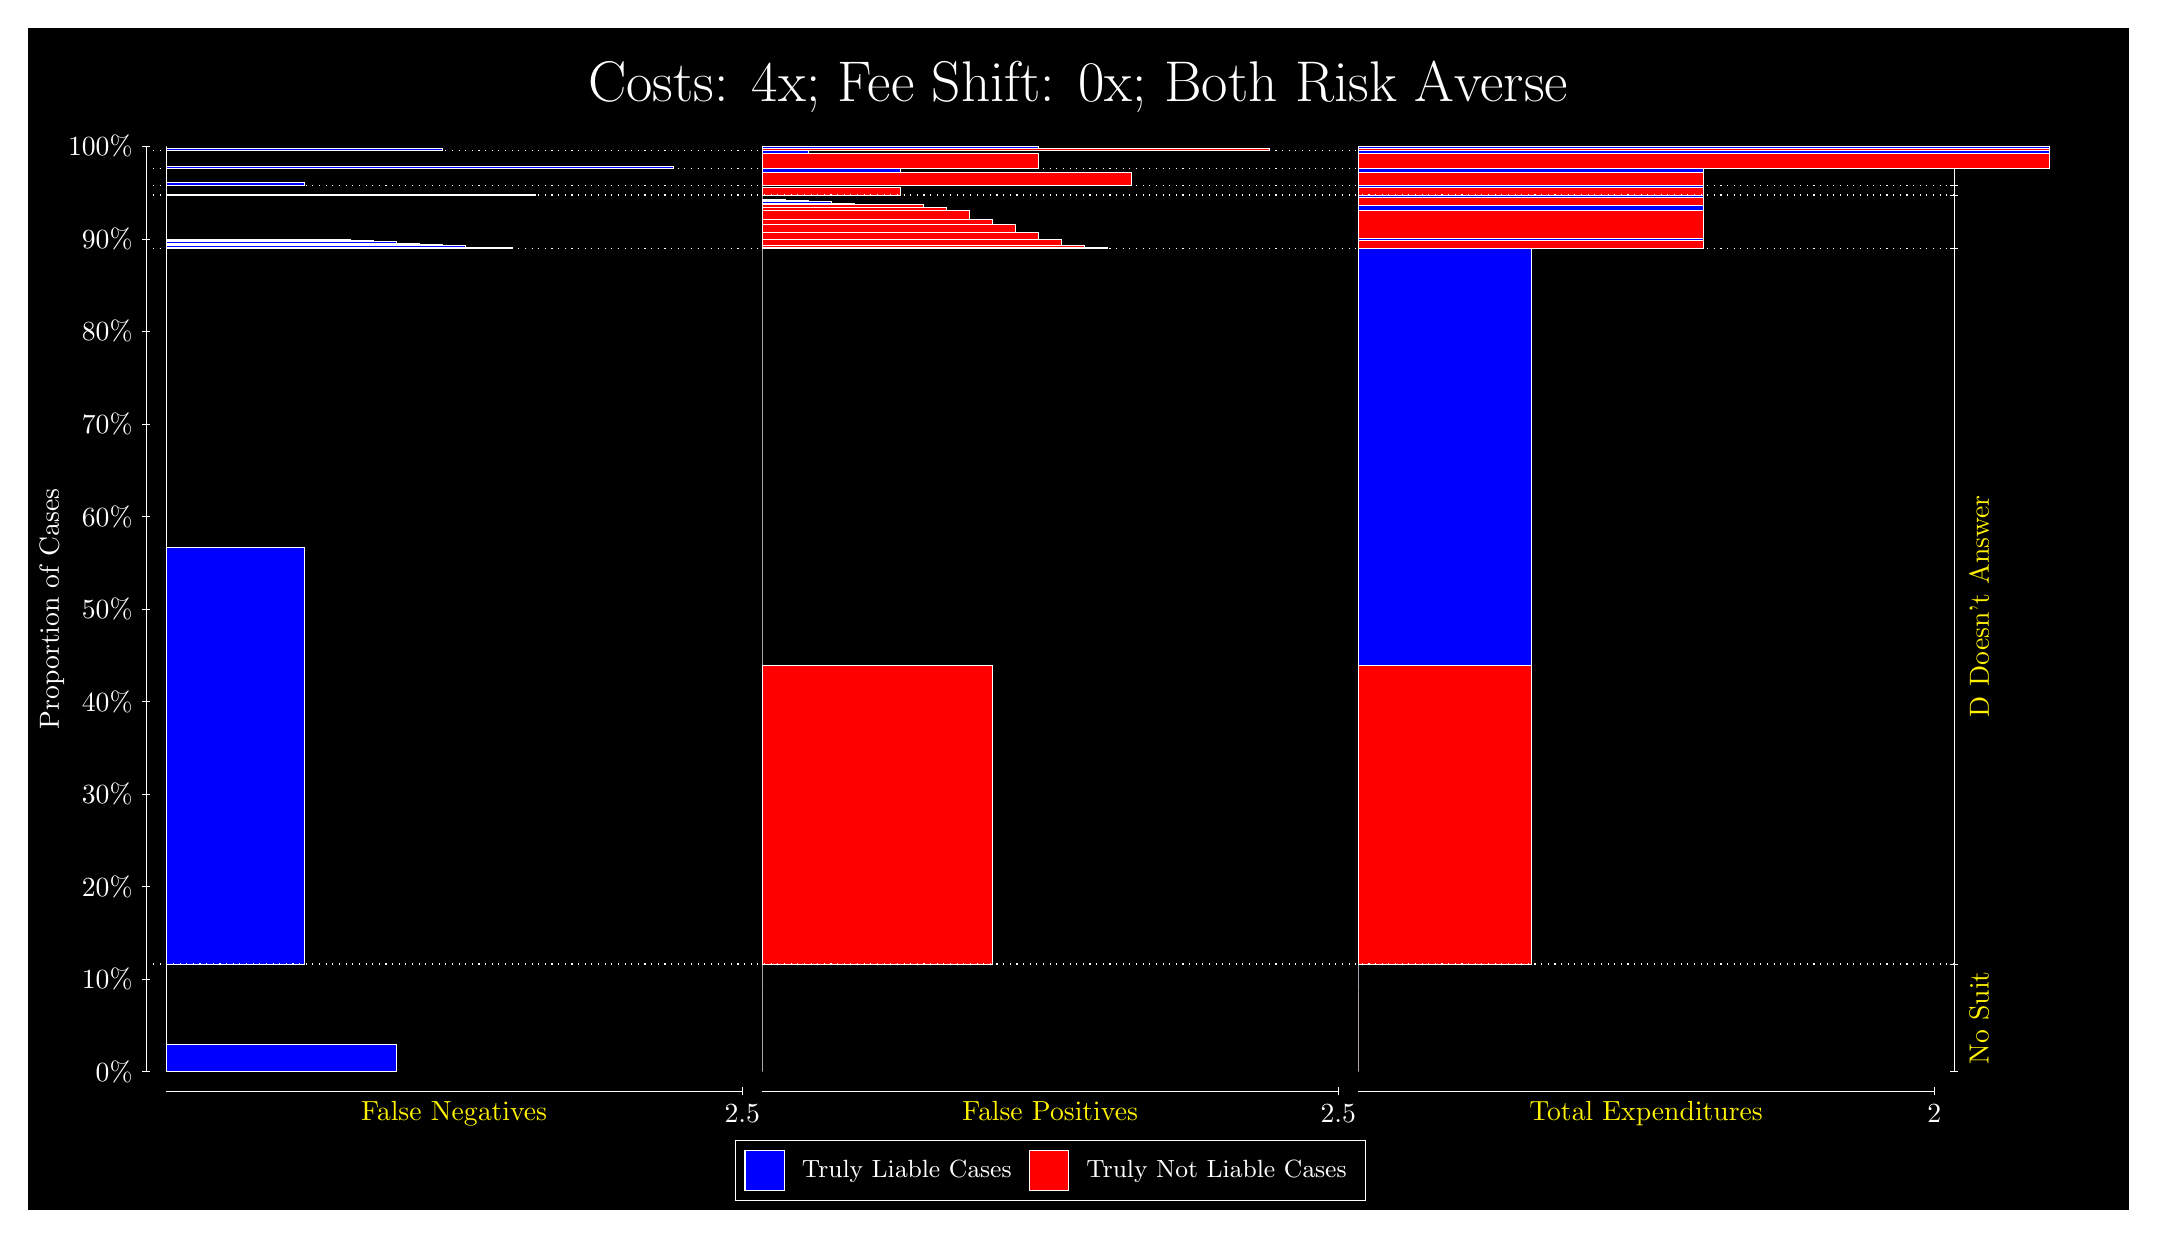
\begin{tikzpicture}
\draw[fill=black] (0,0) rectangle (26.667,15);
\draw[text=white] (0,13.5) rectangle (26.667,15) node[midway] {\huge Costs: 4x; Fee Shift: 0x; Both Risk Averse};
\draw[white, very thin] (1.5,1.75) -- (1.5,13.5);
\node[rotate=90, text=white, anchor=center] at (0.3, 7.625) {Proportion of Cases};
\draw[white, very thin] (1.45,1.75) -- (1.55,1.75);
\node[text=white, anchor=east] at (1.45, 1.75) {0\%};
\draw[white, very thin] (1.45,2.925) -- (1.55,2.925);
\node[text=white, anchor=east] at (1.45, 2.925) {10\%};
\draw[white, very thin] (1.45,4.1) -- (1.55,4.1);
\node[text=white, anchor=east] at (1.45, 4.1) {20\%};
\draw[white, very thin] (1.45,5.275) -- (1.55,5.275);
\node[text=white, anchor=east] at (1.45, 5.275) {30\%};
\draw[white, very thin] (1.45,6.45) -- (1.55,6.45);
\node[text=white, anchor=east] at (1.45, 6.45) {40\%};
\draw[white, very thin] (1.45,7.625) -- (1.55,7.625);
\node[text=white, anchor=east] at (1.45, 7.625) {50\%};
\draw[white, very thin] (1.45,8.8) -- (1.55,8.8);
\node[text=white, anchor=east] at (1.45, 8.8) {60\%};
\draw[white, very thin] (1.45,9.975) -- (1.55,9.975);
\node[text=white, anchor=east] at (1.45, 9.975) {70\%};
\draw[white, very thin] (1.45,11.15) -- (1.55,11.15);
\node[text=white, anchor=east] at (1.45, 11.15) {80\%};
\draw[white, very thin] (1.45,12.325) -- (1.55,12.325);
\node[text=white, anchor=east] at (1.45, 12.325) {90\%};
\draw[white, very thin] (1.45,13.5) -- (1.55,13.5);
\node[text=white, anchor=east] at (1.45, 13.5) {100\%};

\draw[white, very thin] (24.457,1.75) -- (24.457,13.5);
\draw[white, very thin] (24.407,1.75) -- (24.507,1.75);
\node[anchor=west] at (24.407, 1.75) {};
\draw[white, very thin] (24.407,3.1155) -- (24.507,3.1155);
\node[anchor=west] at (24.407, 3.1155) {};
\draw[white, very thin] (24.407,12.205) -- (24.507,12.205);
\node[anchor=west] at (24.407, 12.205) {};
\draw[white, very thin] (24.407,12.882) -- (24.507,12.882);
\node[anchor=west] at (24.407, 12.882) {};
\draw[white, very thin] (24.407,12.999) -- (24.507,12.999);
\node[anchor=west] at (24.407, 12.999) {};
\draw[white, very thin] (24.407,13.216) -- (24.507,13.216);
\node[anchor=west] at (24.407, 13.216) {};
\draw[white, very thin] (24.407,13.444) -- (24.507,13.444);
\node[anchor=west] at (24.407, 13.444) {};
\draw[white, very thin] (24.407,13.5) -- (24.507,13.5);
\node[anchor=west] at (24.407, 13.5) {};

\draw[white, very thin, fill=blue] (1.75,1.75) rectangle (4.6775,2.0991);
\draw[white, very thin, fill=red] (1.75,2.0991) rectangle (1.75,3.1155);
\draw[white, very thin, fill=blue] (1.75,3.1155) rectangle (3.5065,8.4073);
\draw[white, very thin, fill=red] (1.75,8.4073) rectangle (1.75,12.205);
\draw[white, very thin, fill=blue] (1.75,12.205) rectangle (6.1413,12.215);
\draw[white, very thin, fill=blue] (1.75,12.215) rectangle (5.8486,12.223);
\draw[white, very thin, fill=blue] (1.75,12.223) rectangle (5.5558,12.241);
\draw[white, very thin, fill=blue] (1.75,12.241) rectangle (5.2631,12.253);
\draw[white, very thin, fill=blue] (1.75,12.253) rectangle (4.9703,12.274);
\draw[white, very thin, fill=blue] (1.75,12.274) rectangle (4.6775,12.289);
\draw[white, very thin, fill=blue] (1.75,12.289) rectangle (4.3848,12.308);
\draw[white, very thin, fill=blue] (1.75,12.308) rectangle (4.092,12.32);
\draw[white, very thin, fill=blue] (1.75,12.32) rectangle (3.7993,12.323);
\draw[white, very thin, fill=red] (1.75,12.323) rectangle (1.75,12.882);
\draw[white, very thin, fill=blue] (1.75,12.882) rectangle (6.4341,12.895);
\draw[white, very thin, fill=red] (1.75,12.895) rectangle (1.75,12.999);
\draw[white, very thin, fill=blue] (1.75,12.999) rectangle (3.5065,13.045);
\draw[white, very thin, fill=red] (1.75,13.045) rectangle (1.75,13.216);
\draw[white, very thin, fill=blue] (1.75,13.216) rectangle (8.1906,13.246);
\draw[white, very thin, fill=red] (1.75,13.246) rectangle (1.75,13.444);
\draw[white, very thin, fill=blue] (1.75,13.444) rectangle (5.2631,13.471);
\draw[white, very thin, fill=red] (1.75,13.471) rectangle (1.75,13.5);
\draw[white, very thin, fill=red] (9.3189,1.75) rectangle (9.3189,2.7664);
\draw[white, very thin, fill=blue] (9.3189,2.7664) rectangle (9.3189,3.1155);
\draw[white, very thin, fill=red] (9.3189,3.1155) rectangle (12.246,6.9131);
\draw[white, very thin, fill=blue] (9.3189,6.9131) rectangle (9.3189,12.205);
\draw[white, very thin, fill=red] (9.3189,12.205) rectangle (13.71,12.217);
\draw[white, very thin, fill=red] (9.3189,12.217) rectangle (13.417,12.246);
\draw[white, very thin, fill=red] (9.3189,12.246) rectangle (13.125,12.316);
\draw[white, very thin, fill=red] (9.3189,12.316) rectangle (12.832,12.403);
\draw[white, very thin, fill=red] (9.3189,12.403) rectangle (12.539,12.51);
\draw[white, very thin, fill=red] (9.3189,12.51) rectangle (12.246,12.575);
\draw[white, very thin, fill=red] (9.3189,12.575) rectangle (11.954,12.687);
\draw[white, very thin, fill=red] (9.3189,12.687) rectangle (11.661,12.724);
\draw[white, very thin, fill=red] (9.3189,12.724) rectangle (11.368,12.763);
\draw[white, very thin, fill=blue] (9.3189,12.763) rectangle (10.783,12.767);
\draw[white, very thin, fill=blue] (9.3189,12.767) rectangle (10.49,12.778);
\draw[white, very thin, fill=blue] (9.3189,12.778) rectangle (10.197,12.798);
\draw[white, very thin, fill=blue] (9.3189,12.798) rectangle (9.9044,12.813);
\draw[white, very thin, fill=blue] (9.3189,12.813) rectangle (9.6116,12.833);
\draw[white, very thin, fill=blue] (9.3189,12.833) rectangle (9.3189,12.882);
\draw[white, very thin, fill=red] (9.3189,12.882) rectangle (11.075,12.986);
\draw[white, very thin, fill=blue] (9.3189,12.986) rectangle (9.3189,12.999);
\draw[white, very thin, fill=red] (9.3189,12.999) rectangle (14.003,13.171);
\draw[white, very thin, fill=blue] (9.3189,13.171) rectangle (11.075,13.216);
\draw[white, very thin, fill=red] (9.3189,13.216) rectangle (12.832,13.414);
\draw[white, very thin, fill=blue] (9.3189,13.414) rectangle (9.9044,13.444);
\draw[white, very thin, fill=red] (9.3189,13.444) rectangle (15.759,13.473);
\draw[white, very thin, fill=blue] (9.3189,13.473) rectangle (12.832,13.5);
\draw[white, very thin, fill=red] (16.888,1.75) rectangle (16.888,2.7664);
\draw[white, very thin, fill=blue] (16.888,2.7664) rectangle (16.888,3.1155);
\draw[white, very thin, fill=red] (16.888,3.1155) rectangle (19.083,6.9131);
\draw[white, very thin, fill=blue] (16.888,6.9131) rectangle (19.083,12.205);
\draw[white, very thin, fill=red] (16.888,12.205) rectangle (21.279,12.312);
\draw[white, very thin, fill=blue] (16.888,12.312) rectangle (21.279,12.332);
\draw[white, very thin, fill=red] (16.888,12.332) rectangle (21.279,12.685);
\draw[white, very thin, fill=blue] (16.888,12.685) rectangle (21.279,12.751);
\draw[white, very thin, fill=red] (16.888,12.751) rectangle (21.279,12.851);
\draw[white, very thin, fill=blue] (16.888,12.851) rectangle (21.279,12.882);
\draw[white, very thin, fill=red] (16.888,12.882) rectangle (21.279,12.986);
\draw[white, very thin, fill=blue] (16.888,12.986) rectangle (21.279,12.999);
\draw[white, very thin, fill=red] (16.888,12.999) rectangle (21.279,13.171);
\draw[white, very thin, fill=blue] (16.888,13.171) rectangle (21.279,13.216);
\draw[white, very thin, fill=red] (16.888,13.216) rectangle (25.67,13.414);
\draw[white, very thin, fill=blue] (16.888,13.414) rectangle (25.67,13.444);
\draw[white, very thin, fill=red] (16.888,13.444) rectangle (25.67,13.473);
\draw[white, very thin, fill=blue] (16.888,13.473) rectangle (25.67,13.5);
\draw[white, dotted] (1.5,3.1155) -- (24.457,3.1155);
\draw[white, dotted] (1.5,12.205) -- (24.457,12.205);
\draw[white, dotted] (1.5,12.882) -- (24.457,12.882);
\draw[white, dotted] (1.5,12.999) -- (24.457,12.999);
\draw[white, dotted] (1.5,13.216) -- (24.457,13.216);
\draw[white, dotted] (1.5,13.444) -- (24.457,13.444);
\draw[white, very thin] (1.75,1.5) -- (9.0689,1.5);
\node[text=yellow, anchor=north] at (5.4094, 1.5) {False Negatives};
\draw[white, very thin] (9.0689,1.45) -- (9.0689,1.55);
\node[text=white, anchor=north] at (9.0689, 1.45) {2.5};

\draw[white, very thin] (9.3189,1.5) -- (16.638,1.5);
\node[text=yellow, anchor=north] at (12.978, 1.5) {False Positives};
\draw[white, very thin] (16.638,1.45) -- (16.638,1.55);
\node[text=white, anchor=north] at (16.638, 1.45) {2.5};

\draw[white, very thin] (16.888,1.5) -- (24.207,1.5);
\node[text=yellow, anchor=north] at (20.547, 1.5) {Total Expenditures};
\draw[white, very thin] (24.207,1.45) -- (24.207,1.55);
\node[text=white, anchor=north] at (24.207, 1.45) {2};

\node[text=yellow, centered, rotate=90] at (24.777, 2.4327) {No Suit};
\node[text=yellow, centered, rotate=90] at (24.777, 7.6602) {D Doesn't Answer};






\draw (12.978300999999998,1.5) node[draw=none] (baseCoordinate) {};
\begin{scope}[align=center]
        \matrix[scale=0.5, draw=white, below=0.5cm of baseCoordinate, nodes={draw}, column sep=0.1cm]{
            \node[rectangle, draw, minimum width=0.5cm, minimum height=0.5cm, fill=blue] {}; &
            \node[draw=none, font=\small, text=white] (B) {Truly Liable Cases}; &
            \node[rectangle, draw, minimum width=0.5cm, minimum height=0.5cm, fill=red] {}; &
            \node[draw=none, font=\small, text=white] (B) {Truly Not Liable Cases}; \\
            };
\end{scope}

\end{tikzpicture}
\end{document}